% \section{Appendix}

\clearpage
\section{Limitations}
\label{appendix:limits}
In this section, we discuss the potential limitations of the proposed VLA-Cache: 
(i) In dynamic environments with substantial background or object motion, the number of non-reusable tokens increases, reducing acceleration gains. As visualized in Figure~\ref{fig:sim_visual_redundancy}, dynamic regions (highlighted in yellow) require full recomputation. 
(ii) Our experiments focus on three state-of-the-art open-source VLA architectures (OpenVLA~\cite{kim24openvla}, CogAct~\cite{li2024cogact}, OpenVLA-OFT~\cite{kim2025fine}) based on LLaMA2~\cite{touvron2023llama} decoders. The applicability of VLA-Cache to emerging VLA systems with different backbones (e.g., Gemma2~\cite{team2024gemma} in $\pi_0$~\cite{black2024pi_0}) or more complex VLA systems remains an open direction for future work.

\section{Impact Statement}
\label{app:impact}
While VLA-Cache demonstrates robust performance even under dynamic conditions, we emphasize the importance of careful deployment and continuous monitoring to ensure safe, interpretable, and reliable behavior in real-world robotic systems.

\section{Complexity Analysis Details}
\label{appendix:complexity}

\noindent
\textbf{Static Token Selection.} 
We compute patch-wise similarity for visual tokens:
\begin{equation}
\label{eq:patch_sim_flops}
\text{FLOPs}_{\text{static-sim}} = N_{\mathrm{patch}}^2 D_{\mathrm{patch}} \approx H^2.
\end{equation}
Since $N_{\mathrm{patch}} = H/p$, this cost remains small relative to Transformer computations.

\noindent
\textbf{Task-Relevance Filtering.} 
The attention-based filtering step computes cross-modal importance scores:
\begin{equation}
\label{eq:task_relevance_flops}
\text{FLOPs}_{\text{task-filter}} \approx L_t L_v D.
\end{equation}
A sorting operation of $\mathcal{O}(L \log L)$ follows for threshold selection.

\noindent
\textbf{Layer-Adaptive Entropy Computation.} 
The entropy-based reuse strategy involves:
\begin{equation}
\label{eq:entropy_cost}
\text{FLOPs}_{\text{entropy}} \approx L^2 D.
\end{equation}
The per-layer reuse ratio is then computed as:
\begin{equation}
\label{eq:reuse_ratio_append}
\alpha^l = \min\Bigl( k \sum_{j=1}^l R^j, 1 \Bigr).
\end{equation}
These overheads remain modest compared to the full forward pass cost, enabling efficient token reuse.

\noindent
\textbf{Final FLOP Reduction.} 
The total FLOP savings across all layers follow:
\begin{equation}
\label{eq:total_flop_savings}
\Delta \text{FLOPs}_{\text{total}} = \sum_{l=1}^{\Omega} \Delta \text{FLOPs}_{\text{layer}}.
\end{equation}
This confirms that dynamic token reuse significantly reduces computation without sacrificing model performance.

% \section{Inference Details and Implementation}
\section{Inference Detail of VLA-Cache}
\label{app:inference_detail}
\paragraph{Inference Procedure.}
VLA-Cache accelerates robotic action prediction by reusing static visual tokens across frames during inference. At each timestep \( t \), current visual tokens \( \mathbf{H}_t \) are compared with those from the previous frame to identify unchanged regions. Tokens that are both visually static and task-irrelevant are reused via cached key-value (KV) entries, while task-relevant or dynamic tokens are recomputed. This selective reuse substantially reduces visual processing cost without altering model architecture or training.

\paragraph{Token Reuse Mechanism.}
Our implementation modifies the VLA decoder’s forward pass as follows:
\begin{itemize}
    \item \textbf{Position and Attention Masking.} We maintain a \texttt{cache\_position} array to mark tokens requiring recomputation. Static tokens retain their previous position encodings, allowing attention masks to be pruned to match the reduced token set.
    \item \textbf{Rotary Embedding.} For recomputed tokens, rotary embeddings are applied to introduce positional information. Tokens that are skipped retain their previous encoded states.
    \item \textbf{Dynamic Cache Updates.} Newly computed tokens update their respective \(\{\mathbf{K}_t^l, \mathbf{V}_t^l\}\) entries, while reused tokens inherit values from the previous frame’s cache \(\{\mathbf{K}_{t-1}^l, \mathbf{V}_{t-1}^l\}\). Due to the permutation invariance of Transformers, this partial update yields valid attention results.
\end{itemize}
This strategy is fully compatible with standard KV caching in autoregressive decoding. The largest computational gain occurs when generating the first action token at each timestep; subsequent tokens are decoded autoregressively without additional cost.

\paragraph{Experimental Settings.}
All experiments are conducted using OpenVLA with 256 visual tokens. Unless specified otherwise, we use a static token similarity threshold \( \tau = 0.996 \), top-\(k = 100\) for retained static tokens, and a task-relevance threshold \( \tau_{\text{task}} = 0.5 \). These parameters are applied consistently across all simulated and real-world settings, including SIMPLER with CogAct. For real-world Jaco2 experiments, we slightly reduce the similarity threshold to \( \tau = 0.85 \) to accommodate environmental noise. Training on the real robot used LoRA-based fine-tuning for 50,000 steps, and all evaluations were performed on an NVIDIA RTX 4090 GPU.

\section{More Experiment Results}

\subsection{Simulation Experiment}

\paragraph{LIBERO Task Definitions.}
Similarly, we also utilize all task suites provided in LIBERO for our evaluations. The Robosuite-based robot setup includes the following tasks: 1) ``place bowl on plate with {spatial variation}'' (e.g., drawer positions), 2) ``pick {object}'' (e.g., ketchup, bowl, apple), 3) ``(open / close) {target} drawer; {action} {object}'' (e.g., ``open top drawer; place apple into drawer''), and 4) ``achieve {goal} using shared objects'' (e.g., rearranging spatial relationships or altering object states).

\paragraph{SIMPLER Task Definitions.}
We utilize all task variants provided in SIMPLER for our evaluations, which include the Google robot setup with the following tasks: 1) ``pick Coke can'', 2) ``move {obj1} near {obj2}'', 3) ``(open / close) (top / middle / bottom) drawer'', and 4) ``open top drawer; place apple into top drawer''. Evaluations for the Google robot setup are provided for both Visual Matching (VM) and Variant Aggregations (VA).

\paragraph{Implementation Details.} Simulated evaluations for CogACT and SIMPLER are conducted on a single NVIDIA RTX 4090 GPU in BF16 precision. During inference, we use DDIM sampling with 10 steps and a classifier-free guidance (CFG) coefficient of 1.5. Similarly, for OpenVLA and LIBERO, inference is performed on a single NVIDIA RTX 4090 GPU in BF16 precision.
\subsection{Additional Simulation Results}


\paragraph{Result of Subtask on LIBERO Spatial Task Suit.}
Table~\ref{tab:libero_spatial} presents detailed results on each subtask in the LIBERO-Spatial suite. We observe that VLA-Cache, along with methods like SparseVLM and FastV, occasionally surpasses the baseline’s success rate on individual subtasks. This suggests that certain redundant tokens may distract the baseline model, and pruning or reusing tokens can in fact enhance its robustness.
\begin{table*}[h]
\centering
\caption{Comparison of success rates across different tasks in the LIBERO-Spatial benchmark.}
\resizebox{\linewidth}{!}{
\begin{tabular}{lcccccccccccccc}
\toprule
\multirow{2}{*}{Method} 
  & \multicolumn{11}{c}{Success Rate \% $\uparrow$} 
  & \multirow{2}{*}{FLOPs $\downarrow$} 
  & \multirow{2}{*}{CUDA Time (ms) $\downarrow$} \\
\cmidrule(lr){2-12}
& 1 & 2 & 3 & 4 & 5 & 6 & 7 & 8 & 9 & 10 & Avg & & \\ 
\midrule
Baseline (OpenVLA) & 90 & 90 & 84 & 96 & 70 & 90 & 96 & 76 & 82 & 70 & 84.4 & 1.888 & 52.37 \\
SparseVLM          & 88 & 60 & 90 & 90 & 60 & 82 & 90 & \textbf{92} & 72 & \textbf{74} & 79.8 & 1.367 & 88.08 \\
FastV              & \textbf{92} & \textbf{90} & \textbf{90} & \textbf{94} & 58 & \textbf{92} & 90 & 80 & \textbf{78} & 70 & 83.4 & 1.888 & 54.00 \\
\textbf{VLA-Cache} & 90 & \textbf{90} & 88 & \textbf{94} & \textbf{66} & 84 & \textbf{94} & 84 & 76 & 72 & \textbf{83.8} & \textbf{1.382} & \textbf{32.22} \\
\bottomrule
\end{tabular}
}
\vskip -0.05in
\label{tab:libero_spatial}
\end{table*}


\begin{table}[!h]
\centering
\caption{Real-world \textit{PickPot} task under dynamic background (human/object motion).}
\vskip 0.1in
\label{tab:real_robot_dynamic}

\begin{tabular}{lccc}
\toprule
Method & Success (\%) $\uparrow$ & FLOPs $\downarrow$ & Latency (ms) $\downarrow$ \\
\midrule
Baseline (OpenVLA) & 95 & 1.800 & 68.03 \\
+ Noise            & 80 & 1.807 & 68.22 \\
+ Noise, VLA-Cache & 80 & \textbf{1.275} & \textbf{50.59} \\
\bottomrule
\end{tabular}

\end{table}


\paragraph{Visualization Results.}
Figure \ref{fig:simulate_test_traj} present evaluation examples of each tasks executed by OpenVLA with VLA-Cache in LIBERO. More visualized results are available in the supplementary materials.
\begin{figure}[!h]
    \centering
    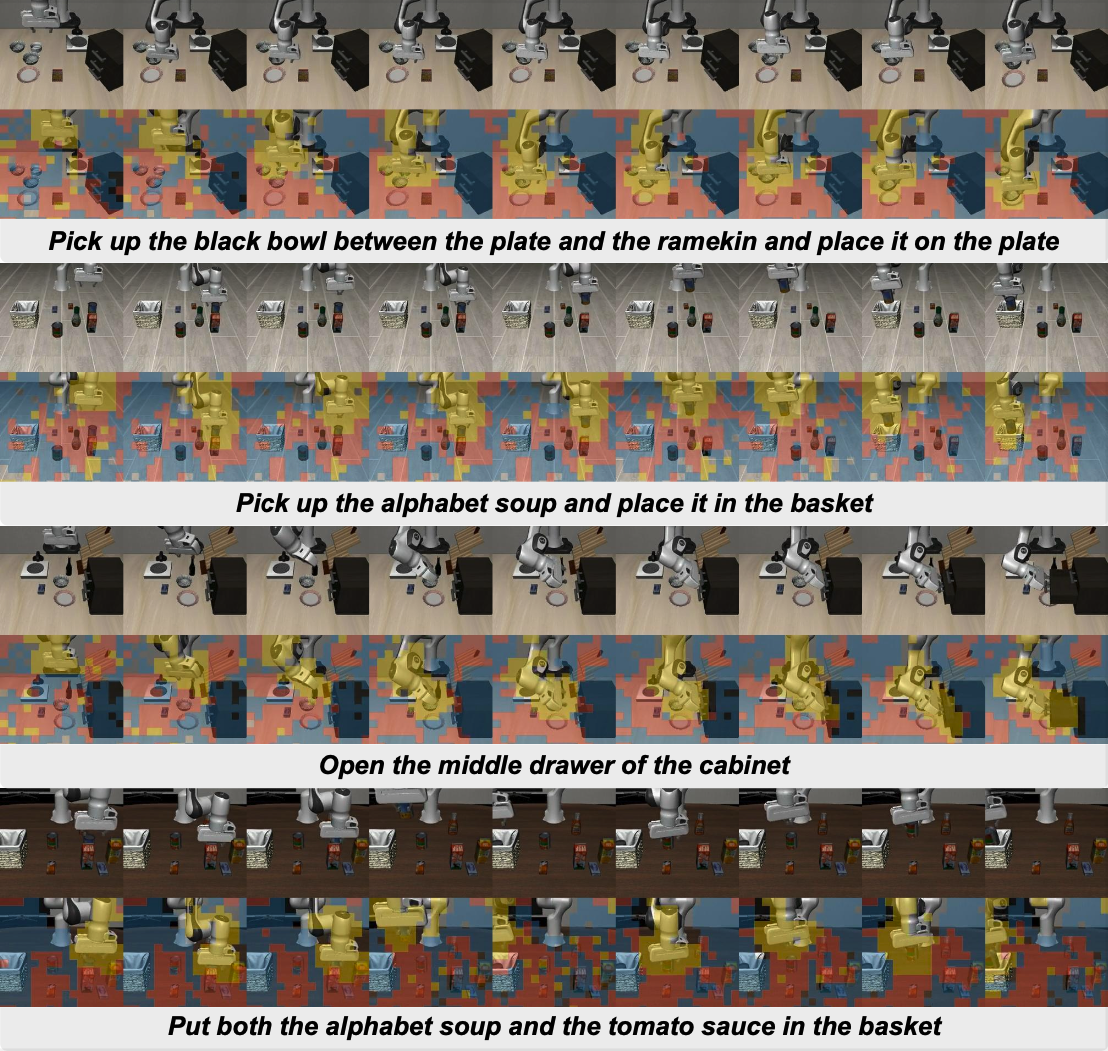
\includegraphics[width=1.0\linewidth]{fig/simulate_test_traj.png}
    \caption{VLA-Cache test results and attention heat map in a simulated environment}
    \label{fig:simulate_test_traj}
\end{figure}

\subsection{Additional Ablations and Comparisons}
\label{sec:add-ablations}

\paragraph{Attention vs.\ object–mask proxies for task relevance.}
To validate whether attention score is a reliable proxy for task relevance, we compared our default attention–based filtering with an object-mask alternative using \emph{Efficient Track Anything}\cite{xiong2024efficient}. On LIBERO-Spatial with OpenVLA-OFT, attention-based proxy yields both higher success rate and lower latency than the mask variant:

\begin{table}[h]
\centering
\setlength{\tabcolsep}{8pt}
\begin{tabular}{lcccc}
\toprule
Method & SR (\%) $\uparrow$ & FLOPs(T) $\downarrow$ & Latency (ms) $\downarrow$ & Freq.\ (Hz) $\uparrow$ \\
\midrule
\textsc{OpenVLA-OFT} & 97.8 & 3.99 & 78.35 & 65.44 \\
\quad + VLA-Cache (Attention) & \textbf{98.3} & \textbf{3.04} & \textbf{61.12} & \textbf{81.67} \\
\quad + VLA-Cache (Object Mask) & 87.4 & 3.15 & 87.49 & 64.78 \\
\bottomrule
\end{tabular}   
\caption{Attention vs.\ object-mask proxies for task relevance on \textsc{LIBERO-Spatial}.}
\label{tab:attn_vs_mask}
\end{table}

While object masks provide spatial localization, they can miss fine-grained or contextual signals essential for manipulation, especially with background clutter or small, relevant parts. In contrast, attention scores are dynamically produced and tightly coupled with the model’s internal reasoning, providing a lightweight, task-adaptive proxy for relevance.

\paragraph{Sensitivity to static-token budget $k$ and relevance threshold $\tau$.}
We further analyze the trade-off between accuracy and efficiency by varying the number of static tokens $k$ (with $\tau{=}0.5$ fixed) and the task-relevance threshold $\tau$ (with $k{=}100$ fixed) on LIBERO-Spatial using OpenVLA-OFT. Results indicate robustness across a wide range; our default $(k{=}100,\ \tau{=}0.5)$ offers a strong balance.

\begin{table}[h]
\centering
\setlength{\tabcolsep}{8pt}
\begin{tabular}{lcccc}
\toprule
Method & SR (\%) $\uparrow$ & FLOPs (T) $\downarrow$ & Latency (ms) $\downarrow$ & Freq.\ (Hz) $\uparrow$ \\
\midrule
\textsc{OpenVLA-OFT} & 97.8 & 3.995 & 78.35 & 65.44 \\
\quad + VLA-Cache ($k{=}50$)  & 97.6 & 3.332 & 66.82 & 77.23 \\
\quad + VLA-Cache ($k{=}80$)  & 97.8 & 3.226 & 66.55 & 78.66 \\
\quad + VLA-Cache ($k{=}100$) & \textbf{98.2} & 3.156 & 64.88 & 79.88 \\
\quad + VLA-Cache ($k{=}120$) & 98.0 & 3.109 & 62.99 & 80.56 \\
\quad + VLA-Cache ($k{=}150$) & 97.4 & \textbf{3.043} & \textbf{61.12} & \textbf{81.67} \\
\quad + VLA-Cache ($k{=}180$) & 96.6 & 2.936 & 60.46 & 82.51 \\
\bottomrule
\end{tabular}
\caption{Varying the static-token budget $k$ (with $\tau{=}0.5$).}
\label{tab:k_sweep}
\end{table}

\begin{table}[h]
\centering
\setlength{\tabcolsep}{8pt}
\begin{tabular}{lcccc}
\toprule
Method & SR (\%) $\uparrow$ & FLOPs (T) $\downarrow$ & Latency (ms) $\downarrow$ & Freq.\ (Hz) $\uparrow$ \\
\midrule
\textsc{OpenVLA-OFT} & 97.8 & 3.995 & 78.35 & 65.44 \\
\quad + VLA-Cache ($\tau{=}0.2$) & 95.6 & 3.384 & 66.93 & 76.74 \\
\quad + VLA-Cache ($\tau{=}0.3$) & 96.2 & 3.283 & 67.03 & 79.31 \\
\quad + VLA-Cache ($\tau{=}0.4$) & 98.0 & 3.204 & 66.38 & 79.79 \\
\quad + VLA-Cache ($\tau{=}0.5$) & \textbf{98.2} & 3.156 & 64.88 & 79.88 \\
\quad + VLA-Cache ($\tau{=}0.6$) & 98.6 & 3.131 & 64.27 & 81.98 \\
\quad + VLA-Cache ($\tau{=}0.7$) & 98.4 & \textbf{3.068} & \textbf{63.12} & \textbf{82.96} \\
\bottomrule
\end{tabular}
\caption{Varying the relevance threshold $\tau$ (with $k{=}100$).}
\label{tab:tau_sweep}
\end{table}

\noindent
Overall, efficiency (FLOPs and latency) improves monotonically with larger $k$ and $\tau$, while success rate remains consistently high, corroborating the stability of \emph{VLA-Cache} across sensitivity settings. Our default $(k{=}100,\ \tau{=}0.5)$ is used for all main results unless stated otherwise.

\paragraph{Applicability to diffusion-based and alternative VLA architectures.}
\emph{VLA-Cache} is designed to accelerate the language-decoder stage of VLAs and is therefore not directly applicable to models without a vision–language backbone, such as standalone diffusion policies. However, for hybrid architectures that combine a VLM with a diffusion-based policy head (e.g., CogACT~\cite{li2024cogact}), our method remains fully compatible and has shown consistent efficiency gains and stable task performance in the SIMPLER environment, as shown in Table \ref{tab:simpler_eval}. Since \emph{VLA-Cache} operates by reusing temporally static visual tokens before action generation, it can be integrated with diffusion-based or transformer-style models (e.g., RDT, DiT) that exhibit inter-frame redundancy, offering a promising direction for future generalization.

\subsection{Real Robot Experiment}
\label{app:realworld_details}
\paragraph{Robot Setup.}
The setup of the Franka Robot is shown in Figure ~\ref{fig:real_robot}. In this example, a Kinova Jaco robot arm with 6 degrees of freedom is rigidly fixed to the frame. We use a Sony AX53 camera, which is placed opposite the robot arm. The camera is facing the operating table and transmits the video in real time.

\begin{figure}[h] 
    \centering
    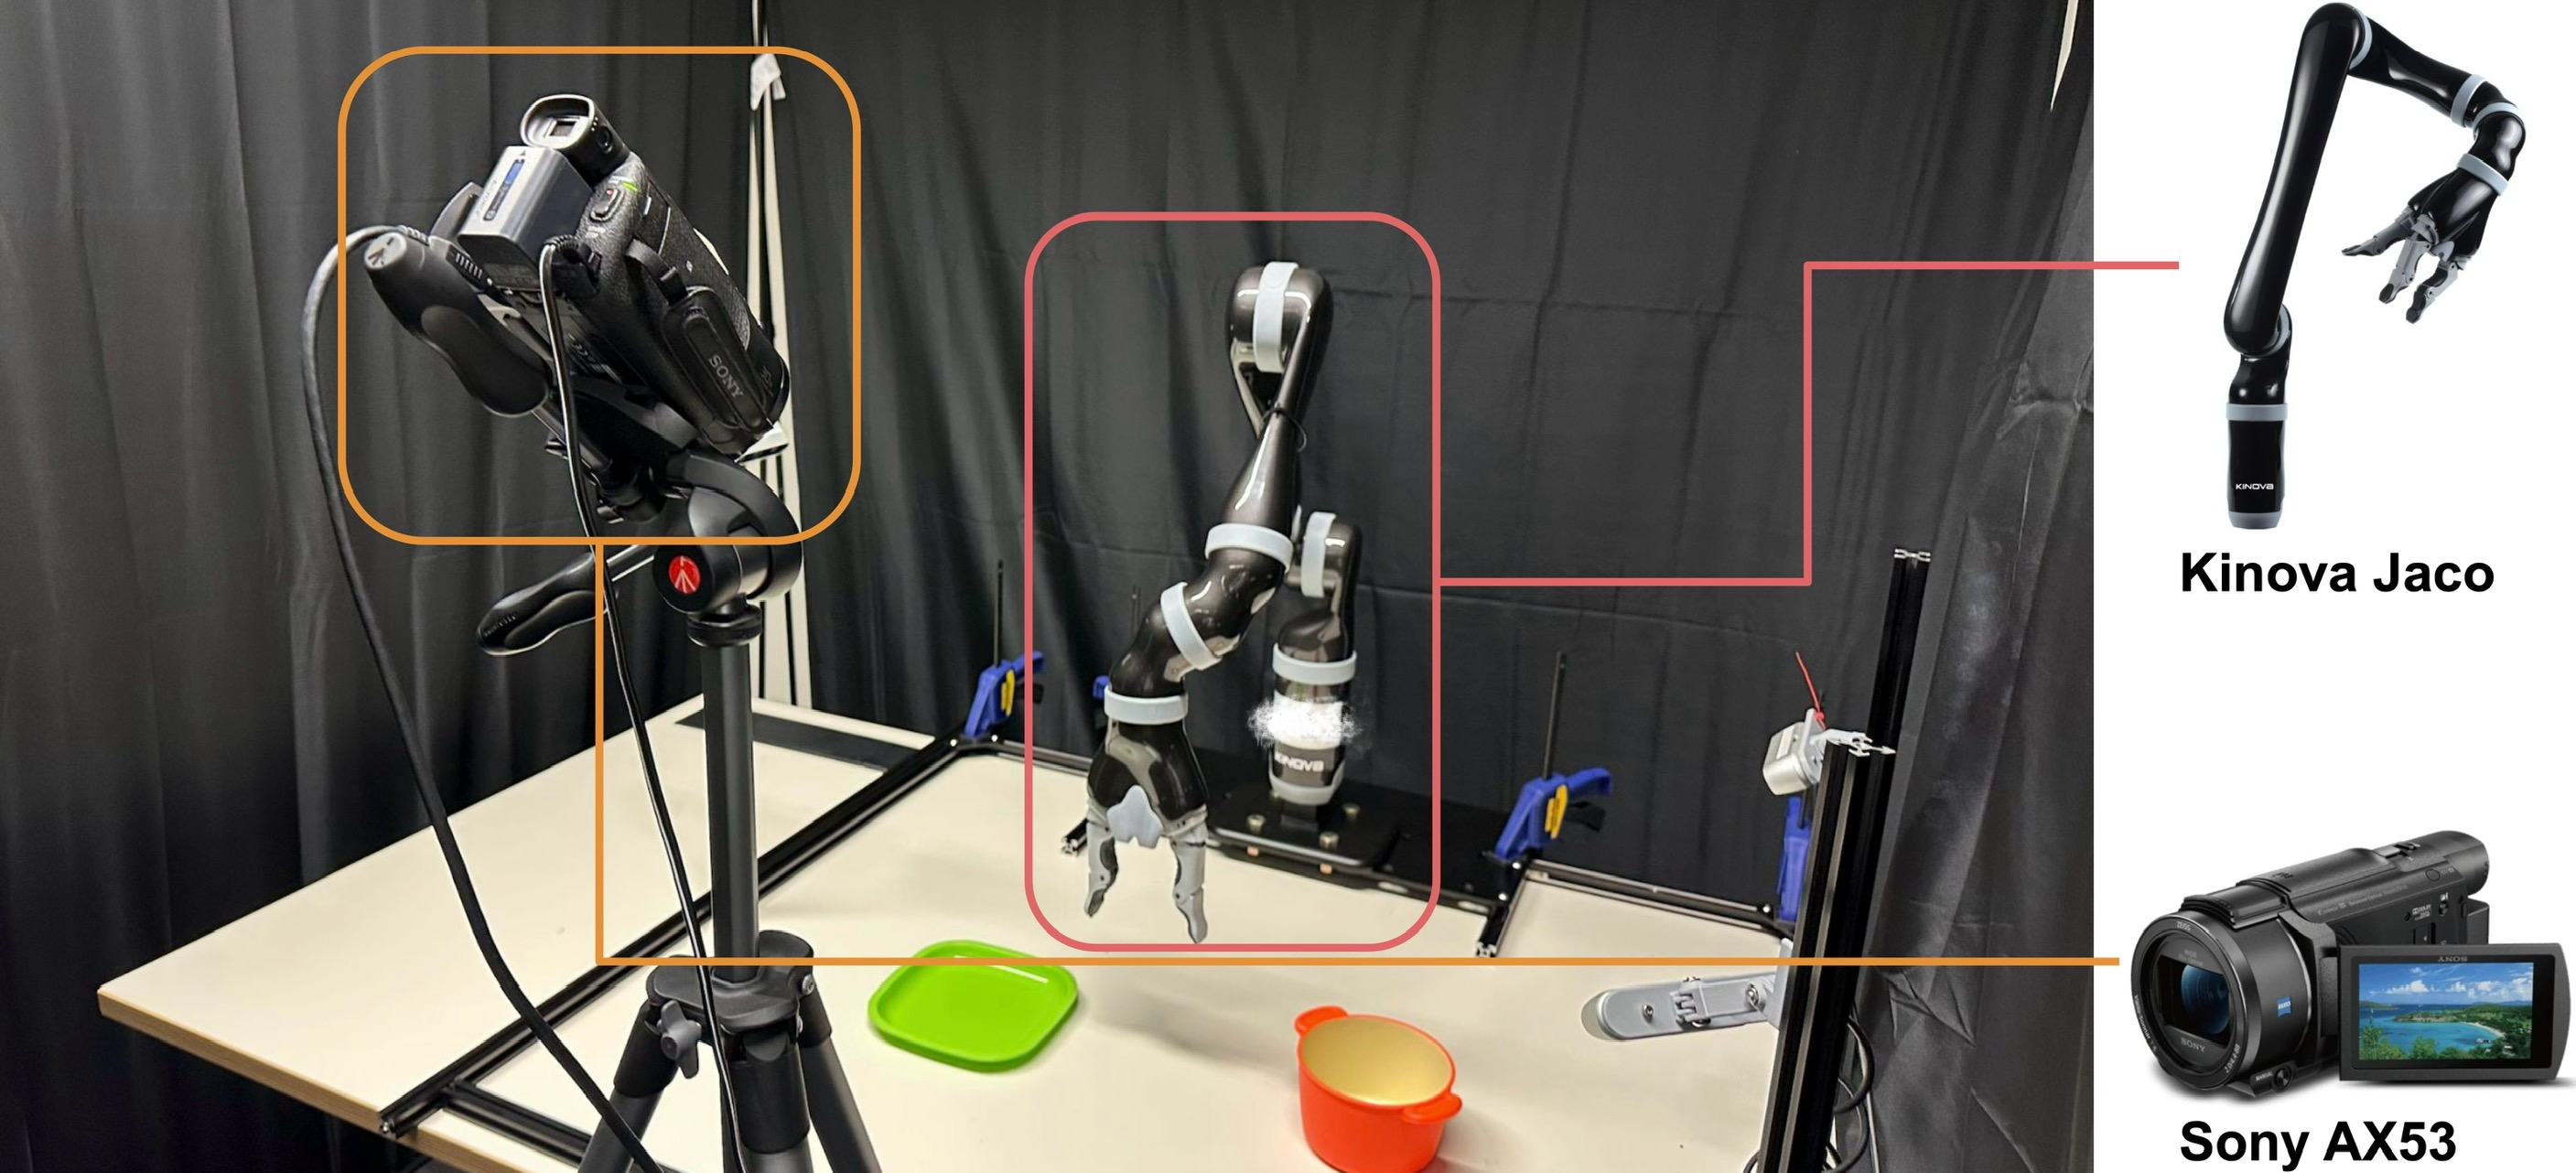
\includegraphics[width=0.8\linewidth]{fig/real_robot.jpg} 
    \caption{Kinova Jaco Robot Setup}
    \label{fig:real_robot}
\end{figure}

\paragraph{Data Collection.}
Our data collection work is based on the \textit{CLVR\_Jaco\_Play} dataset. We employed PyBullet as an inverse kinematics (IK) controller. The system receives incremental Cartesian displacement inputs ($\Delta x, \Delta y, \Delta z$) from an Xbox controller, which are processed to generate joint velocity commands. These commands are transmitted to the robotic arm\textquotesingle s velocity controller at a 10Hz control frequency for real-time execution. We record four types of observations: Third-person camera observations (\textbf{front\_cam\_ob}), End-effector Cartesian pose (\textbf{ee\_cartesian\_pos\_ob}), End-effector Cartesian velocity (\textbf{ee\_cartesian\_vel\_ob}), Jaco arm joint positions (\textbf{joint\_pos\_ob}).


\paragraph{Data Preprocessing.}
The preprocessing procedure was conducted as follows. Initially, the recorded frames underwent center cropping, reducing the resolution from 1280$\times$720 to 912$\times$720, followed by resizing to 224$\times$224. Subsequently, episodes were manually selected based on a visual inspection of the video sequences generated from the recorded frames. To minimize potential biases associated with excessively long episodes, those exceeding 250 steps were excluded from the dataset. Furthermore, steps in which all recorded action values were zero were removed to ensure data relevance and integrity.

\paragraph{Task Definitions and Success Criteria.}
We design four single-instruction tasks for the real-world robot setting to evaluate manipulation performance across diverse object types and interaction modes. The task definitions are as follows:
\begin{enumerate}
    \item \textbf{Pick Up Orange Pot} (PickPot): The robot\textquotesingle s goal is to grasp the orange pot and lift it completely off the table. A trial is successful if the pot is grasped and raised with visible clearance from the surface. We collected 218 valid demonstrations for the training dataset, with slight random adjustments to the initial positions of the pot and the robotic arm in each episode. During evaluation, each trial is recorded as a success (1) or failure (0); there is no partial credit.
    \item \textbf{Place Blue Cube in Box} (PlaceCube): The robot\textquotesingle s goal is to place the held blue cube into the target container. A trial is successful if the cube is fully inside the container at the terminal step without contact-induced ejection. We collected 212 valid demonstrations for the training dataset, with randomized container positions and robotic arm initial configurations in each episode. During evaluation, each trial is recorded as a success (1) or failure (0); there is no partial credit.
    \item \textbf{Put Sausage in Blue Pan} (PutSausage): The robot\textquotesingle s goal is to stably place the held sausage into the blue pan. Success requires the sausage to rest inside the pan boundary at the terminal step. We collected 219 valid demonstrations for the training dataset, with randomized pan coordinates and robotic arm joint angles across trials. During evaluation, each trial is recorded as a success (1) or failure (0); there is no partial credit.
    \item \textbf{Wipe Table} (WipeTable): The robotic arm\textquotesingle s goal is to sweep scattered items into a fixed-position dustpan using a broom. Success requires all designated items to be inside the dustpan area at termination. For the training dataset, we collected 187 valid demonstrations featuring randomized placements of simulated items (e.g., fries/cheese) on the table and varied initial joint configurations of the robotic arm, while the dustpan location remained fixed. This task explicitly incorporates dynamic environmental variations to rigorously test generalization capabilities. During evaluation, each trial is recorded as a success (1) or failure (0); there is no partial credit.
\end{enumerate}


\paragraph{Trial Protocol and Randomization.}
We run \textbf{20} trials for \emph{PickPot} and \emph{PutSausage}, and \textbf{30} trials for \emph{PlaceCube} and \emph{WipeTable}, for a total of \textbf{100} trials per method. For each trial we randomize the initial robot configuration and the object placement within a bounded region of the workspace. Trials are single-attempt with a fixed horizon; there is no human intervention or reset within a trial. Outcomes are recorded as binary success or failure per the criteria above.

\begin{table}[h]
\centering
\setlength{\tabcolsep}{10pt}
\begin{tabular}{lcccccc}
\toprule
& \multicolumn{3}{c}{\textsc{OpenVLA}} & \multicolumn{3}{c}{\textsc{OpenVLA} + \textsc{VLA-Cache}} \\
\cmidrule(lr){2-4}\cmidrule(lr){5-7}
Task & Success & Failure & SR (\%) & Success & Failure & SR (\%) \\
\midrule
PickPot (20)     & 19 & 1 & 95.0 & 18 & 2 & 90.0 \\
PlaceCube (30)   & 25 & 5 & 83.3 & 27 & 3 & 90.0 \\
PutSausage (20)  & 16 & 4 & 80.0 & 17 & 3 & 85.0 \\
WipeTable (30)   & 21 & 9 & 70.0 & 22 & 8 & 73.3 \\
\midrule
\textbf{Total (100)} & 81 & 19 & 82.1 & 84 & 16 & 84.6 \\
\bottomrule
\end{tabular}
\caption{Real-world results with trial counts and success rates.}
\label{tab:real_counts}
\end{table}
\paragraph{Results with Counts and Rates.}
Table~\ref{tab:real_counts} reports per-task successes and failures, along with the corresponding success rate. Average success is computed across all $100$ trials.


\begin{figure}[!h]
    \centering
    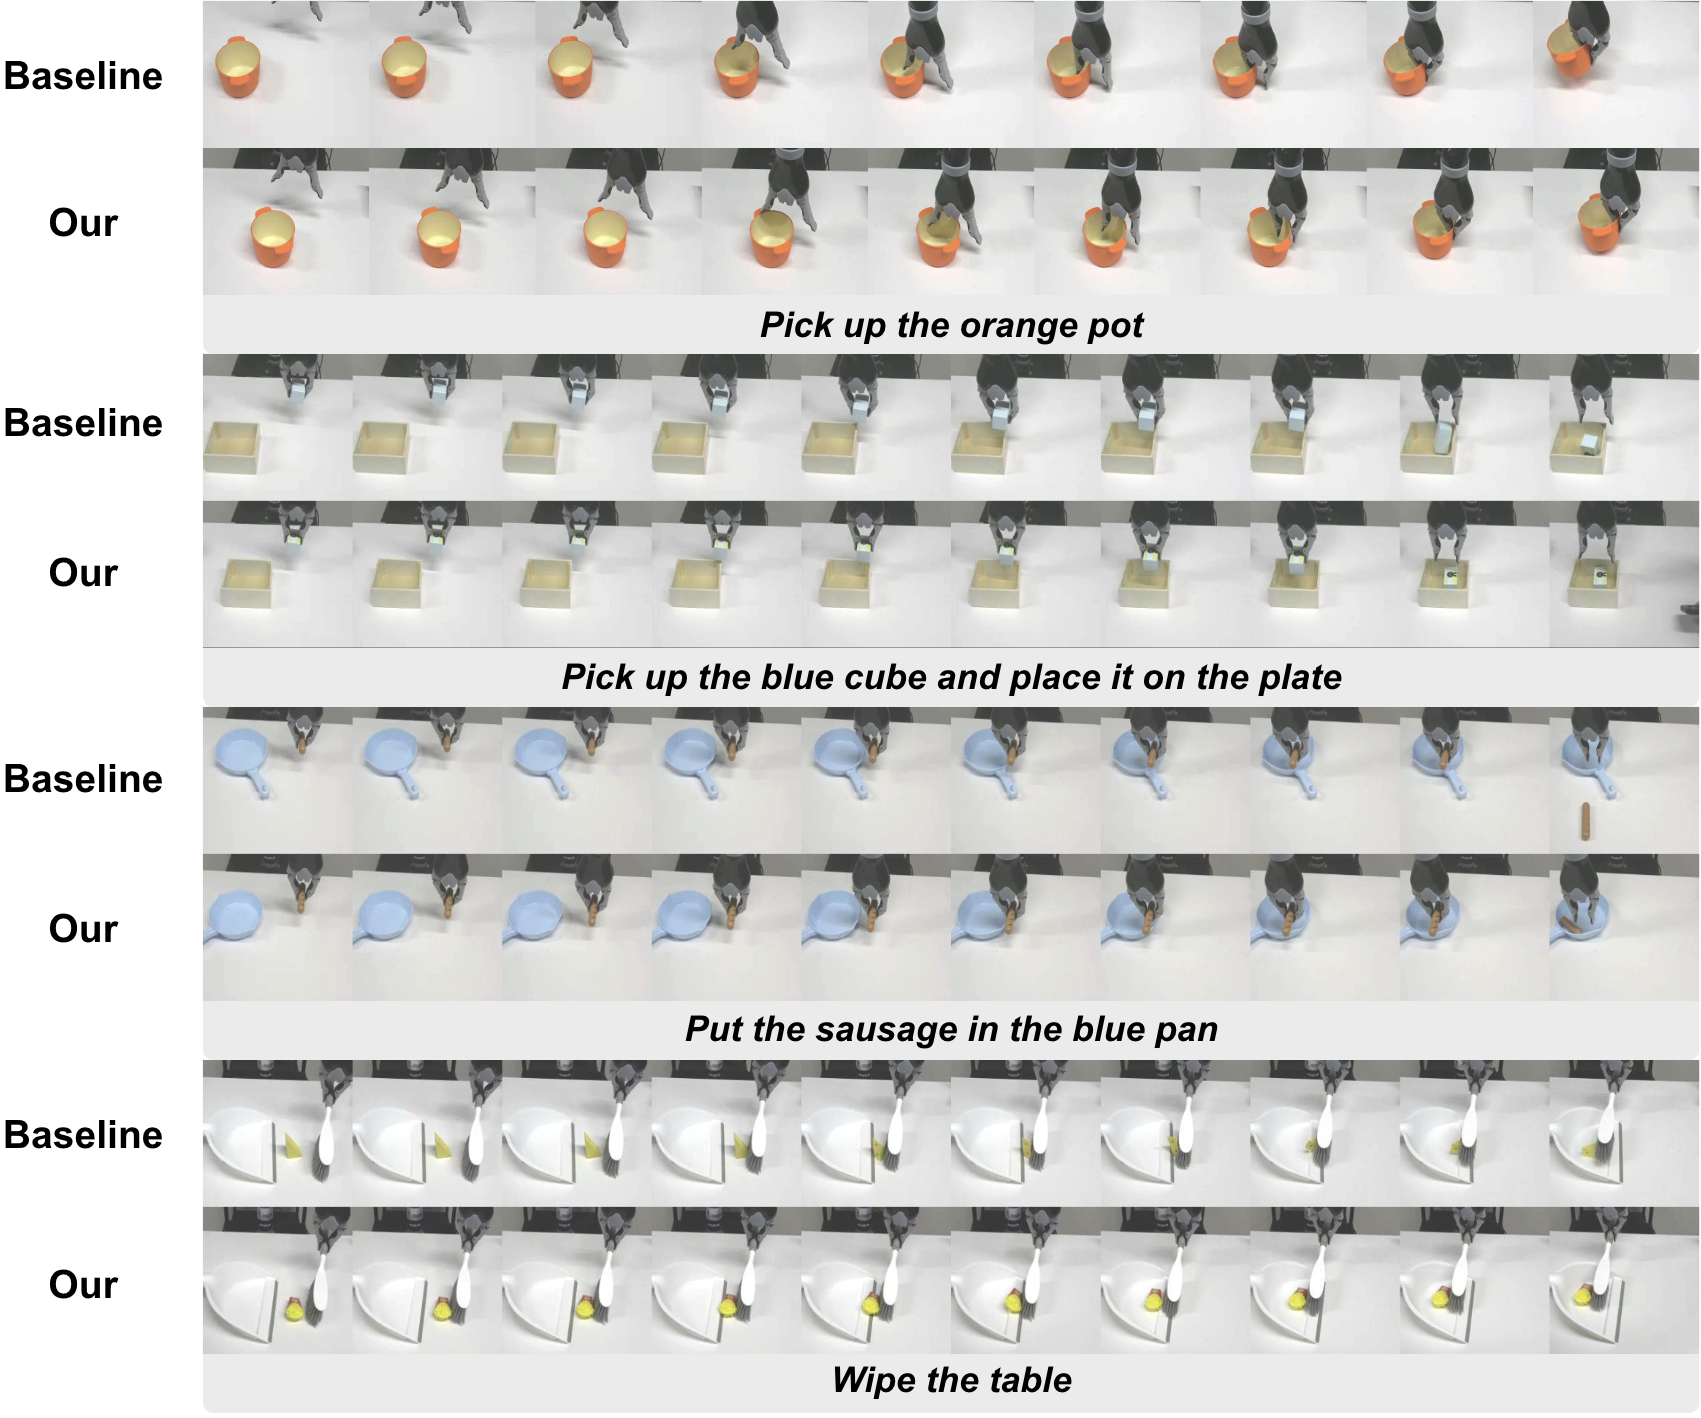
\includegraphics[width=1.0\linewidth]{fig/real_test_traj.png}
    \caption{Comparison between baseline (OpenVLA) and VLA-Cache in real environment.}
    \label{fig:real_test_traj}
\end{figure}
\paragraph{Visualization Results.}
Figure \ref{fig:real_test_traj} present evaluation examples of each tasks executed by OpenVLA with VLA-Cache on the Kinova Jaco Robot Arm. More visualized results are available in the supplementary materials.